\renewcommand{\captiontitle}{\CNN{} 分割错误例子}
\begin{figure*}
\begin{center}

\setlength{\tabcolsep}{1pt}

\begin{tabular}{cccc}

\toprule
\SA{}(顶层切片) & \SA{}(顶层切片) & \HLA{} & \VLA{} \\
\midrule

\multicolumn{4}{c}{未对齐方向的原始图像:$\image$} \\

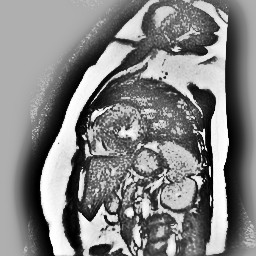
\includegraphics[width=0.19\textwidth]{./data/failures/HCMNet_2000062/00_SAX/9/9.png} &
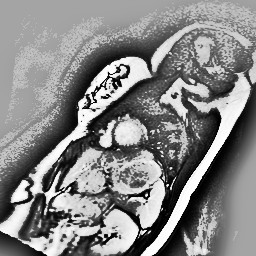
\includegraphics[width=0.19\textwidth]{./data/failures/HCMNet_2400044/00_SAX/2/5.png} &
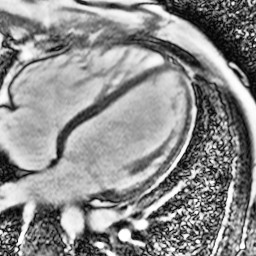
\includegraphics[width=0.19\textwidth]{./data/failures/HCMNet_2600079/01_HLA/00/0.png} &
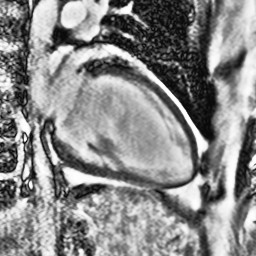
\includegraphics[width=0.19\textwidth]{./data/failures/HCMNet_2600079/02_VLA/00/0.png} \\

\multicolumn{4}{c}{结构定位} \\

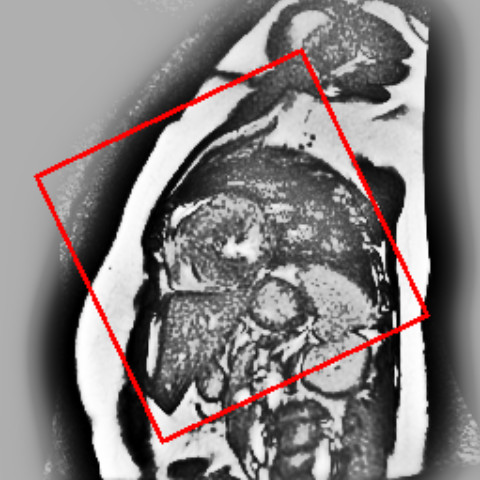
\includegraphics[width=0.19\textwidth]{./data/failures/HCMNet_2000062/00_SAX/9/9_bbox.png} &
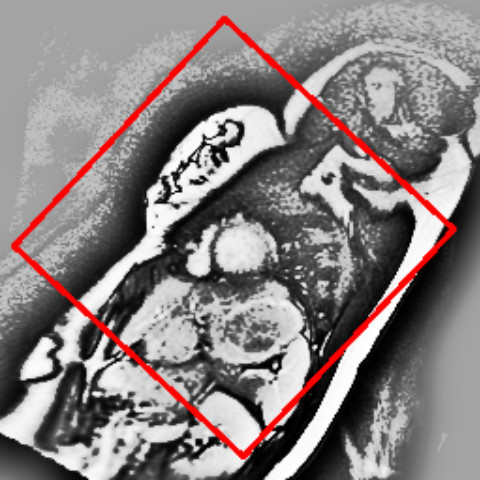
\includegraphics[width=0.19\textwidth]{./data/failures/HCMNet_2400044/00_SAX/2/5_bbox.png} &
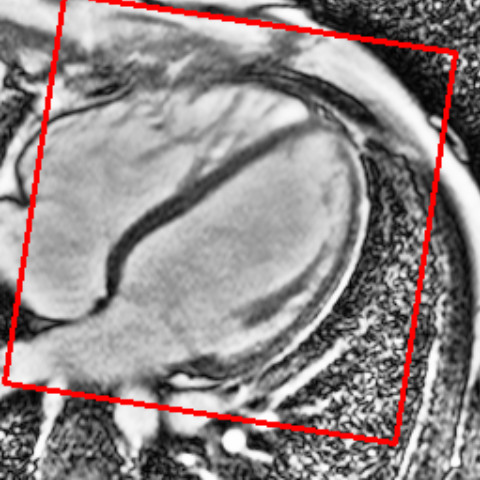
\includegraphics[width=0.19\textwidth]{./data/failures/HCMNet_2600079/01_HLA/00/0_bbox.png} &
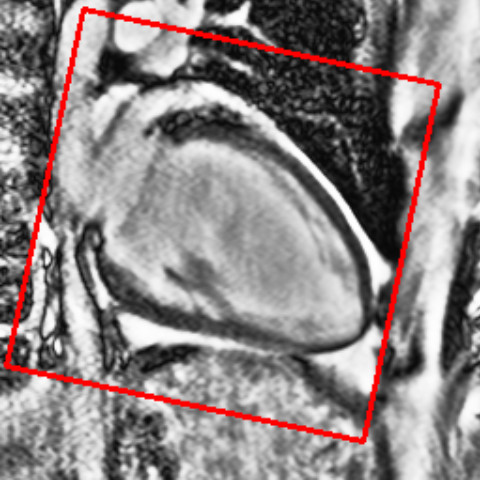
\includegraphics[width=0.19\textwidth]{./data/failures/HCMNet_2600079/02_VLA/00/0_bbox.png} \\

\multicolumn{4}{c}{在典型方向下的分割预测值:$S^\prime$} \\

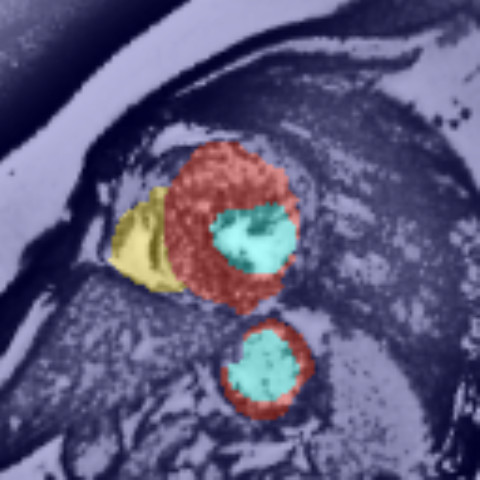
\includegraphics[width=0.19\textwidth]{./data/failures/HCMNet_2000062/00_SAX/9/9_pred.png} &
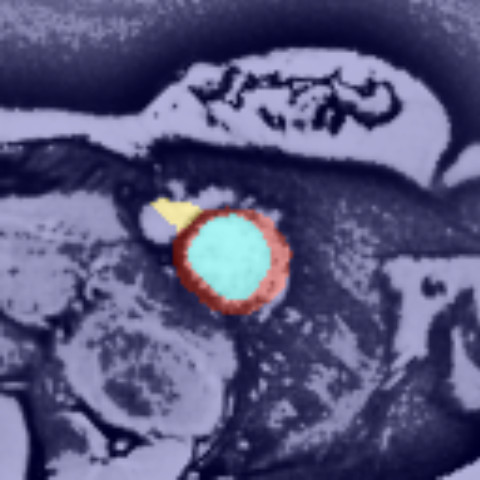
\includegraphics[width=0.19\textwidth]{./data/failures/HCMNet_2400044/00_SAX/2/5_pred.png} &
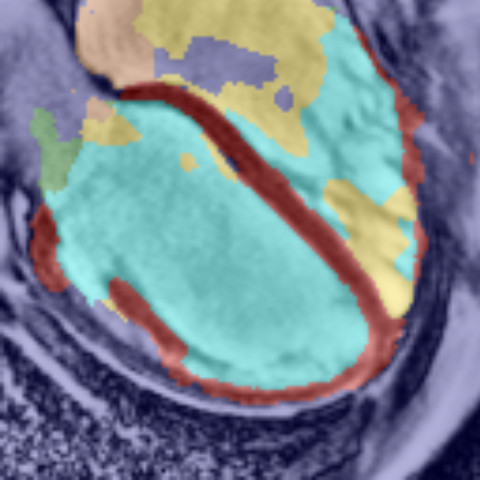
\includegraphics[width=0.19\textwidth]{./data/failures/HCMNet_2600079/01_HLA/00/0_pred.png} &
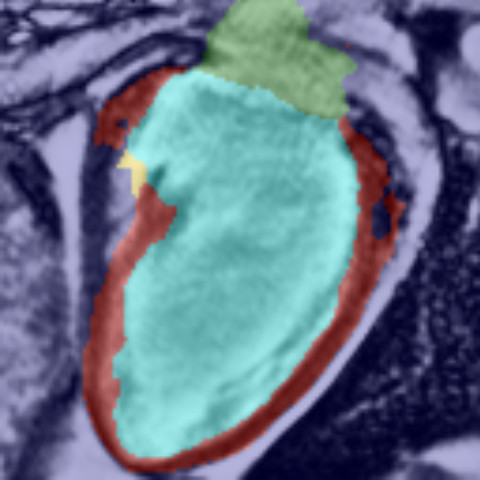
\includegraphics[width=0.19\textwidth]{./data/failures/HCMNet_2600079/02_VLA/00/0_pred.png} \\
\bottomrule

\multicolumn{4}{c}{在典型方向下的分割真实值:$\hat{S}^\prime$} \\

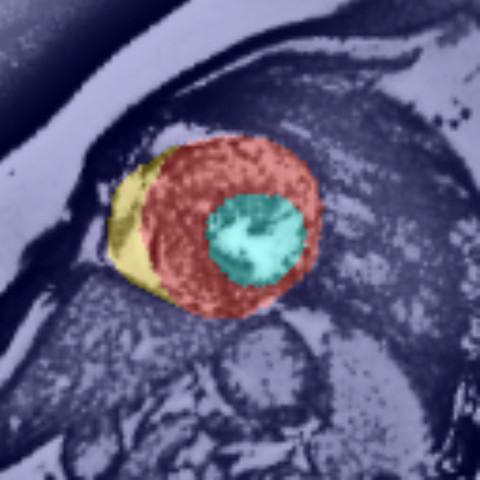
\includegraphics[width=0.19\textwidth]{./data/failures/HCMNet_2000062/00_SAX/9/9_gt.png} &
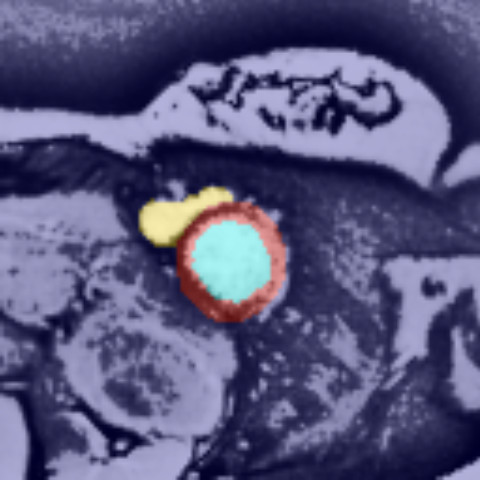
\includegraphics[width=0.19\textwidth]{./data/failures/HCMNet_2400044/00_SAX/2/5_gt.png} &
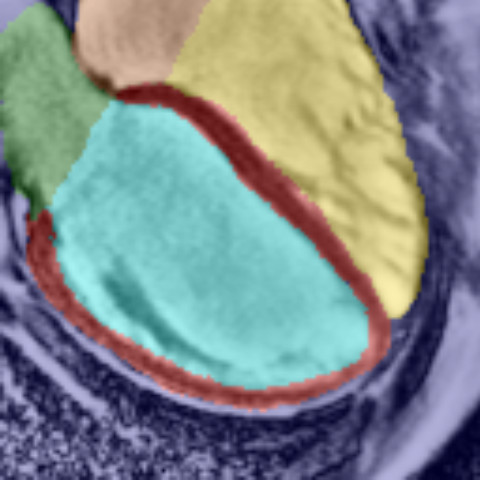
\includegraphics[width=0.19\textwidth]{./data/failures/HCMNet_2600079/01_HLA/00/0_gt.png} &
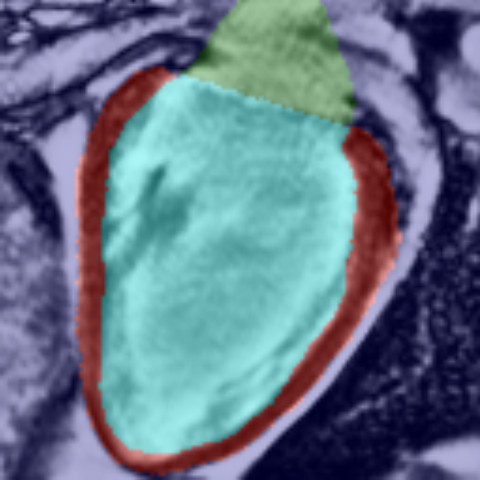
\includegraphics[width=0.19\textwidth]{./data/failures/HCMNet_2600079/02_VLA/00/0_gt.png} \\
\bottomrule

\end{tabular}

\caption[\captiontitle]{\captiontitle{}.详细讨论参考正文.}
\label{fig:failure}
\end{center}
\end{figure*}
